%==============================================================================
% Sjabloon poster bachproef
%==============================================================================
% Gebaseerd op document class `a0poster' door Gerlinde Kettl en Matthias Weiser
% Aangepast voor gebruik aan HOGENT door Jens Buysse en Bert Van Vreckem

\documentclass[a0,portrait]{hogent-poster}

% Info over de opleiding
\course{Bachelorproef}
\studyprogramme{toegepaste informatica}
\academicyear{2023-2024}
\institution{Hogeschool Gent, Valentin Vaerwyckweg 1, 9000 Gent}

% Info over de bachelorproef
\title{Slimme Energiemodellen in de Warmwalserij bij ArcelorMittal}
\subtitle{}
\author{Quintin Mintiens}
\email{quintin.mintiens@student.hogent.be}
\supervisor{Mevr. G. Vercauteren}
\cosupervisor{Dhr. T. De Raad, Dhr. A. Vande Ghinste (ArcelorMittal)}

% Indien ingevuld, wordt deze informatie toegevoegd aan het einde van de
% abstract. Zet in commentaar als je dit niet wilt.
\specialisation{Data Science}
\keywords{energievoorspelling, anomaly detection, machine learning, LSTM}
\projectrepo{https://github.com/user/repo}

\begin{document}

\maketitle

\begin{abstract}
Deze bachelorproef richt zich op het ontwikkelen van slimme energiemodellen voor het detecteren van anomalieën in het energieverbruik van ovens in de warmwalserij van ArcelorMittal. Verschillende machine learning-modellen, met name Long Short-Term Memory (LSTM) netwerken, werden ontwikkeld en geëvalueerd. Het onderzoek toont aan dat LSTM-netwerken effectief zijn in het voorspellen van energieverbruik en het detecteren van afwijkingen, wat bijdraagt aan een efficiënter energiebeheer en kostenbesparing.
\end{abstract}

\begin{multicols}{2} % This is how many columns your poster will be broken into, a portrait poster is generally split into 2 columns

\section{Introductie}

De warmwalserij bij ArcelorMittal verbruikt aanzienlijke hoeveelheden energie. Efficiënt energiebeheer is cruciaal om operationele kosten te verlagen en duurzaamheid te bevorderen. Dit onderzoek richt zich op het ontwikkelen van een model dat energieverbruik nauwkeurig kan voorspellen en anomalieën kan detecteren.

\section{Methodologie}

\subsection{Data Verzameling en Verwerking}
Data werd verzameld uit de operationele databases van ArcelorMittal, inclusief kenmerken zoals datum, gemiddelde breedte en dikte van de slabs, energieverbruik van de ovens, en het totale gewicht van de geproduceerde slabs. Deze data werd genormaliseerd voor uniformiteit.

\subsection{Feature Engineering}
Belangrijke kenmerken zoals productietijd, gemiddelde dikte en breedte van de slabs, en het gewicht van de slabs werden geselecteerd en getransformeerd om de voorspellingskracht van het model te optimaliseren.

\subsection{Modelselectie en Training}
Een Long Short-Term Memory (LSTM) netwerk werd geselecteerd vanwege zijn vermogen om lange termijn afhankelijkheden in tijdreeksdata te leren. Het model werd getraind met een sequence length van 64 tijdstappen, de Adam optimizer, en de Mean Squared Error (MSE) loss functie.

\section{Resultaten}

Het LSTM-model toonde de beste prestaties in het voorspellen van energieverbruik, met een validation loss van 0.023. Dit suggereert een hoge nauwkeurigheid in het identificeren van patronen in energieverbruiksdata en het voorspellen van anomalieën.

\begin{center}
  \captionsetup{type=figure}
  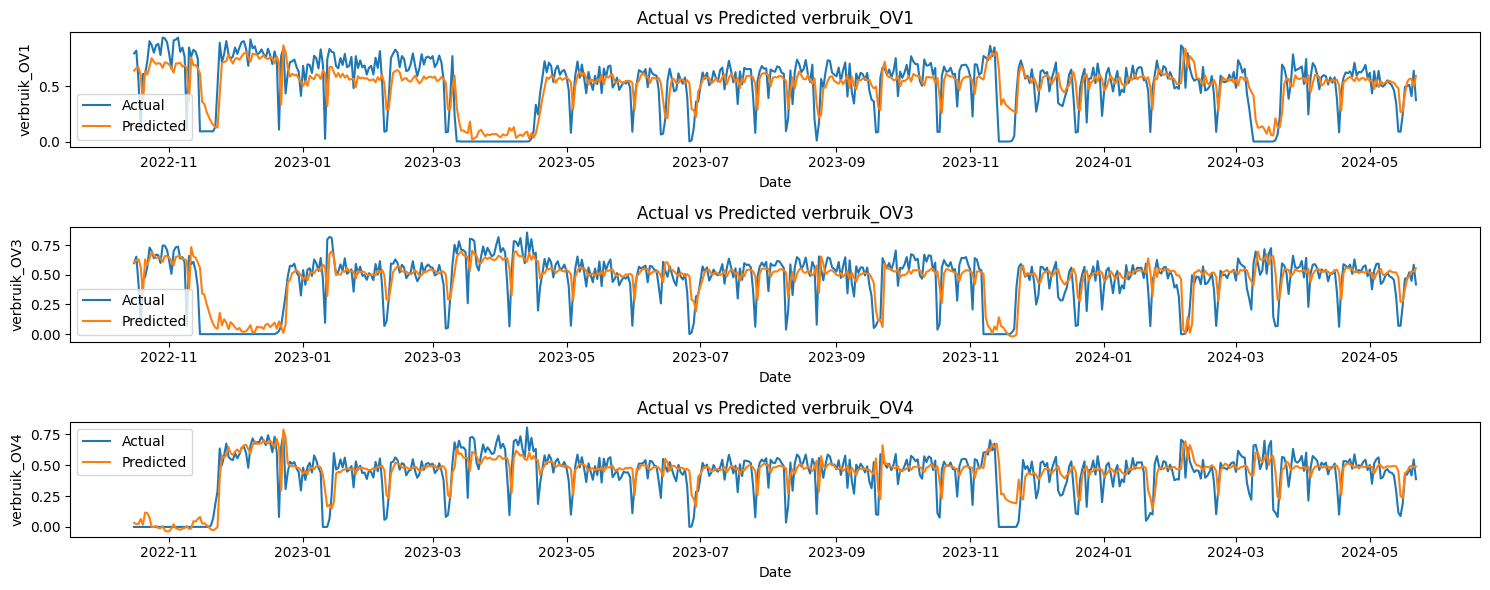
\includegraphics[width=1.0\linewidth]{./graphics/model_performance.png} 
  \captionof{figure}{Modelprestaties: effectief verbruik versus voorspeld verbruik voor alle ovens}
\end{center}

\section{Conclusies}

Het onderzoek bevestigt dat LSTM-netwerken effectief zijn voor het voorspellen van energieverbruik en het detecteren van anomalieën in industriële processen. Dit leidt tot verbeterd energiebeheer, lagere kosten, en ondersteuning van duurzaamheidsinitiatieven bij ArcelorMittal.

\section{Toekomstig Onderzoek}

Toekomstig onderzoek kan zich richten op verdere optimalisatie van het model, uitbreiding naar andere industriële processen, en integratie van real-time data voor nog nauwkeurigere voorspellingen en efficiënter energiebeheer.

\end{multicols}
\end{document}
